\section{Tactile Data Representation and Collection}
\label{sec:data}

If tactile sensors convert contact into signals, the question of how to \emph{structure} those signals, how to \emph{collect} them at scale, and how to build \emph{general-purpose representations} through pretraining defines the data foundation for learned manipulation. This section reviews the representation taxonomy, sensor-agnostic approaches, public datasets, foundation models, and collection pipelines.

\begin{figure}[t]
\centering
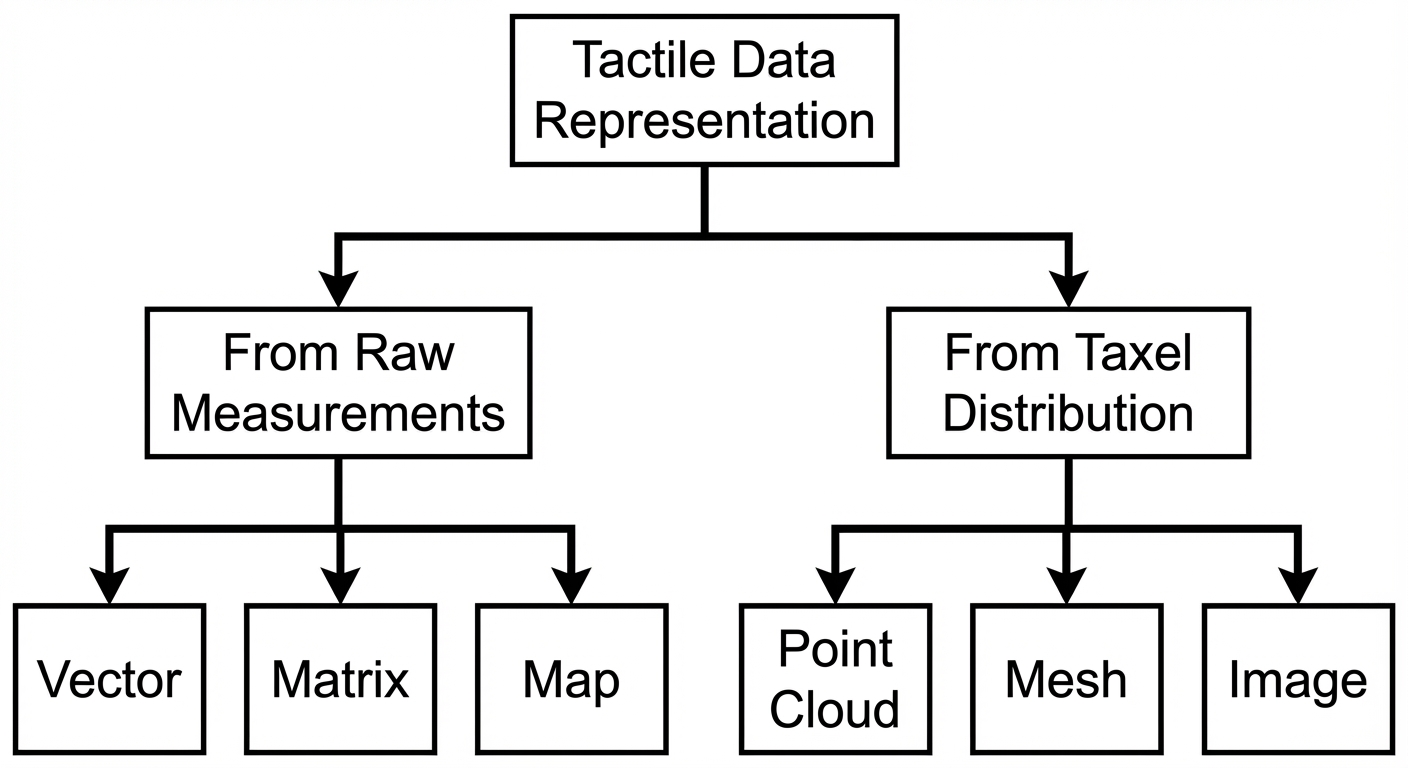
\includegraphics[width=\columnwidth]{../assets/figures/ch03/fig_3_1_albini_taxonomy_academic.png}
\caption{Albini et al.'s six-structure taxonomy of tactile data representations: vector, matrix, map, point cloud, mesh, and image. Selection depends on sensor hardware, task requirements, and information needs.}
\label{fig:albini_taxonomy}
\end{figure}

\subsection{Representation Taxonomy}

Albini et al.~\cite{albini2025representing} (submitted to \emph{IEEE T-RO}) systematized tactile data representations into six canonical structures, providing selection guidelines based on hardware output characteristics, task requirements, and information needs:

\begin{enumerate}
    \item \textbf{Vector}: The simplest form---each sensor's readings arranged as a 1D vector (e.g., OSMO's 36-dimensional force vector from 12 three-axis sensors~\cite{yin2025osmo}). Suitable for classification, force control, and slip detection, but loses spatial relationship information.
    \item \textbf{Matrix}: Sensor array outputs as a 2D grid (e.g., STAG's 548-sensor pressure matrix~\cite{sundaram2019stag}). Natural for contact pattern classification but distorted when sensors are placed on curved surfaces.
    \item \textbf{Map}: Data projected onto a reference surface. UniTacHand~\cite{zhang2025unitachand} projects both human glove and robot tactile data onto MANO UV maps, creating a shared representation space for cross-embodiment transfer (see Section~\ref{sec:retarget}).
    \item \textbf{Point cloud}: Contact points with 3D coordinates. Robot Synesthesia~\cite{yuan2024synesthesia} (ICRA 2024) used PointNet to process tactile point clouds for visuotactile in-hand manipulation, achieving generalization to novel objects including double-ball rotation and 3-axis reorientation.
    \item \textbf{Mesh}: Triangulated contact surfaces for FEM-based deformation simulation. DiffTactile~\cite{si2024difftactile} (ICLR 2024) uses mesh-based contact modeling in a differentiable simulator supporting gradient-based optimization.
    \item \textbf{Image}: The raw output of vision-based tactile sensors is already an image, enabling direct application of CNNs, ViTs, and the full vision model ecosystem. Currently the most widely used representation due to the dominance of GelSight/DIGIT sensors.
\end{enumerate}

The choice of representation directly impacts learning performance. Wu et al.~\cite{wu2025canonical} (ICRA 2025) demonstrated that transforming raw sensor output into a \emph{canonical 3D coordinate frame} enables task-agnostic transfer: a two-stage pipeline of play-data pretraining followed by few-shot expert fine-tuning achieved 78\% average success versus 63\% for T-DEX, representing a 24\% relative improvement from the representation choice alone.

\subsection{Sensor-Agnostic Representations}

A fundamental limitation is \emph{sensor specificity}: representations learned on GelSight do not transfer to DIGIT, and DIGIT representations fail on ReSkin. Three approaches address this challenge, each targeting the ``CLIP moment'' for touch---aligning diverse sensor outputs into a unified embedding space:

\textbf{AnyTouch}~\cite{feng2025anytouch} (ICLR 2025) learns unified static-dynamic representations across multiple vision-based tactile sensors through a multi-level framework, introducing the TacQuad aligned multi-modal multi-sensor dataset.

\textbf{Sensor-Invariant Representation}~\cite{various2025sensorinvariant} achieves zero-shot transfer across optical sensor designs by stripping sensor-specific information while preserving essential contact characteristics.

\textbf{Canonical 3D Tactile}~\cite{wu2025canonical} transforms raw sensor output into a 3D canonical coordinate frame, constructing sensor-independent representations that combine with task-agnostic play data pretraining for efficient transfer.

\subsection{Public Datasets}

The scale of tactile datasets remains orders of magnitude smaller than vision datasets, representing a fundamental bottleneck for foundation model development. Table~\ref{tab:datasets} summarizes major public datasets.

\begin{table}[t]
\caption{Major Tactile Datasets}
\label{tab:datasets}
\centering
\begin{tabular}{@{}L{2.2cm}L{1.8cm}cc@{}}
\toprule
\textbf{Dataset} & \textbf{Scale} & \textbf{Modal.} & \textbf{Year} \\
\midrule
Touch-and-Go~\cite{yang2022touchandgo} & 3M+ contacts & V+T & 2023 \\
Touch100k~\cite{yang2024touch100k} & 100K+ images & T & 2024 \\
VTDexManip~\cite{liu2025vtdexmanip} & 10 tasks, 182 obj. & V+T & 2025 \\
OXE~\cite{oxe2024} & 1M+ traj., 22 emb. & V+A & 2024 \\
\bottomrule
\end{tabular}
\end{table}

VTDexManip~\cite{liu2025vtdexmanip} (ICLR 2025) is a significant milestone---the first large-scale visual-tactile dataset from actual human demonstrations of dexterous manipulation, spanning 10 tasks and 182 objects with an RL benchmark. Open X-Embodiment~\cite{oxe2024} (ICRA 2024) is the largest robot manipulation dataset (1M+ trajectories from 22 embodiments, 34 labs) but includes tactile data in only a small subset. Expanding from Touch-and-Go's 3M contacts to the 100M+ scale needed for robust foundation models remains a key open challenge.

\subsection{Tactile Foundation Models}

Two approaches pursue the ``ImageNet moment'' for touch through self-supervised pretraining:

\textbf{Sparsh}~\cite{higuera2024sparsh} (Meta FAIR/CMU/Berkeley, CoRL 2024) is a self-supervised tactile foundation model pretrained on 460K+ images from multiple vision-based tactile sensors. Its significance lies in being the first large-scale attempt to replicate for touch what ImageNet pretraining accomplished for vision. However, 460K images remain two orders of magnitude below ImageNet's 14M, and a 10$\times$+ expansion is needed for robust generalization.

\textbf{UniTouch}~\cite{yang2024unitouch} (CVPR 2024) uses contrastive learning to align touch with vision, language, and audio into a unified embedding space---analogous to CLIP for vision-language. This enables zero-shot tactile classification and cross-modal retrieval without task-specific fine-tuning, demonstrating that the semantic structure of touch can be captured through alignment with other modalities.

\subsection{Data Collection Pipelines}

Collecting tactile data is inherently harder than visual data because physical contact is required. Four approaches span the throughput-quality trade-off:

\textbf{Teleoperation} yields the highest-quality demonstrations but at $\sim$10 demos/hr throughput. AnyTeleop~\cite{qin2023anyteleop} (RSS 2023) provides general-purpose vision-based dexterous teleoperation via Dex-Retarget. Bunny-VisionPro~\cite{ding2024bunny} achieves research-grade teleoperation using consumer Apple Vision Pro hardware.

\textbf{Portable motion capture}: DexCap~\cite{wang2024dexcap} (Stanford, RSS 2024) achieves 3$\times$ faster data collection than standard teleoperation, with policy learning from just 30 minutes of data.

\textbf{Kinesthetic teaching}: DexForce~\cite{chen2025dexforce} (\emph{IEEE RA-L}) uses a spring model ($x_f = x_o + k_f \cdot f$, single parameter $k_f = 0.0045$) to naturally record force-torque information during physical guidance, capturing richer contact dynamics than teleoperation.

\textbf{Synthetic data}: NVIDIA's Isaac Sim pipeline generates 780K trajectories (equivalent to 6{,}500 hours of real data) in just 11 hours, improving real-world performance by 40\%~\cite{nvidia2025synthetic}. Open-source simulators Tacto~\cite{wang2022tacto} (PyRender + PyBullet for vision-based sensors) and DiffTactile~\cite{si2024difftactile} (differentiable FEM-based contact) enable sim-to-real tactile training.
